\chapter{Livello fisico}

Come riportato nella sezione~\ref{ss:dw-phy}, l'interfaccia tra debug server, l'ATMega16U2, e il controllore target è costituita da una linea seriale open drain.

Si rende necessario quindi implementare tale interfaccia in modo efficiente al fine di permettere al server GDB di interfacciarsi con il \textit{target} tramite DebugWire

\section{Implementazione}

L'implementazione inizialmente progettata in fase di ideazione, ancora prima che fosse stabilita la piattaforma hardware, sfruttava la periferica UART presente sul controllore ATMega16U2\cite[chap. 18]{avr:m16u2}.

Al fine di implementare l'accesso alla linea open drain si rende necessario l'utilizzo di un componente aggiuntivo come mostrato nella figura~\ref{fig:od-impl}, la quale mostra due alternative di implementazione utilizzando un diodo o un transistor. 

\begin{figure}[t]
    \centering

    \subfloat[][]{
        \begin{circuitikz}
            \draw (0, 0) node[label={[font=\footnotesize]above:rxd}] {} to[short, *-] (2, 0) to[short, -] (2, 1) to[R={\(R_{pullup}\)}] (2, 2) to [short, -] (2, 2.5) to [short, -] (2.5, 2.5) to [short, -] (2.5, 3);
            \draw (2.5, 2.5) to[short, -] (3, 2.5) to[short, -] (3, 2) to[R={\(R1\)}] (3, 1);
            \draw (3,-1) node [npn,xscale=-1,anchor=B] (npn) {\reflectbox{\(Q1\)}} (npn.collector);
            \draw (3, 1) to[short, -] (3, -1);
            \draw (2, 0) to[short, *-*] (4, 0) node[label={[font=\footnotesize]above:target}] {};
            \draw (0, -2) node[label={[font=\footnotesize]above:txd}] {} to[short, *-]  (2.16, -2) to[short, -] (2.16, -1.75);
            \draw (2.16, 0) to[short, *-] (2.16, -0.5);
            \draw (2, 3) -- node[anchor=south,align=center] {VCC} (3, 3);
        \end{circuitikz}
    }
    \subfloat[][]{
        \begin{circuitikz}
            \draw (0, 0) node[label={[font=\footnotesize]above:rxd}] {} to[short, *-] (2, 0) to[short, -] (2, 1) to[R={\(R_{pullup}\)}] (2, 2) to [short, -] (2, 3);
            \draw (1.5, 3) -- node[anchor=south,align=center] {VCC} (2.5, 3);
            \draw (2, 0) to[short, *-*] (4, 0) node[label={[font=\footnotesize]above:target}] {};
            \draw (2, 0) to[short, -] (2, -0.5) to[D={\(D1\)}] (2, -1.5) to[short, -] (2, -2)  to [short, -*] (0, -2) node[label={[font=\footnotesize]above:txd}] {};
        \end{circuitikz}
    }
    \caption[]{L'immagine mostra due possibili circuiti per l'adattamento della periferica UART dell'ATMega16U2 alla linea seriale open drain.}\label{fig:od-impl}
\end{figure}

Il principio di funzionamento dei circuiti in figura~\ref{fig:od-impl} è pressoché identico: Il valore del pin txd viene replicato sulla linea di connessione con un livello logico 0 ``forte'' e un livello logico 0 ``debole'' dato dalla resistenza \(R_{pullup}\) e in entrambi i casi il pin txd viene utilizzato come collettore di corrente.
La differenza consiste nella quantità di componenti aggiuntivi e nelle prestazioni.

Il circuito (a) permette, tramite il pin \textit{txd}, di porre la differenza di potenziale \(V_{be}\) tra base ed emettitore del transistor a circa 5V --- ignorando la caduta di tensione irrilevante sulla resistenza R1 --- permettendo una corrente di base sufficiente a mandare il transistor in saturazione. Questo manda il transistor in conduzione, ed essendo in saturazione, porta la differenza di potenziale \(V_{ce}\) a circa 0.2V imponendo così la tensione sulla connessione verso il target.

Contrariamente il circuito (b) sfrutta il diodo D1 per ottenere lo stesso risultato. La differenza consta nel fatto che nel circuito (a) il transistor permette di avere una caduta di tensione minore essendo in saturazione, cosa che avviene quando il segnale \textit{txd} è zero.

I circuiti sopra mostrati sono verificati dalle simulazioni i cui risultati sono mostrati in figura~\ref{graph:sim}. In aggiunta a quanto esibito, il circuito (b) è stato simulato con un diodo schottky 1N5817 con capacitanza di 125pF per valutarne il comportamento.

\begin{figure}
    \centering
        \begin{tikzpicture}
            \begin{axis}[
                width=0.8\textwidth,
                xlabel={Tempo (S)},
                ylabel={Tensione (V)}
                ]
                \addplot table [x=t, y=v(tgt), col sep=comma, mark=none] {sims/phy-sim-bjt.csv};
                \addplot table [x=t, y=v(txd), col sep=comma, mark=none] {sims/phy-sim-bjt.csv};
                \legend{$tgt$,$txd$}
            \end{axis}
        \end{tikzpicture}\\
        \vfill
        \begin{tikzpicture}
            \begin{axis}[
                width=0.8\textwidth,
                xlabel={Tempo (S)},
                ylabel={Tensione (V)}
                ]
                \addplot table [x=t, y=v(tgt), col sep=comma, mark=none] {sims/phy-sim-diode.csv};
                \addplot table [x=t, y=v(txd), col sep=comma, mark=none] {sims/phy-sim-diode.csv};
                \addplot table [x=Time, y=V(NODE1), col sep=comma, mark=none] {sims/phy-sim-schottky.csv};
                \legend{$tgt (pn)$,$txd$}
            \end{axis}
        \end{tikzpicture}
    \caption[]{Risultati della simulazione dei circuiti in figura~\ref{fig:od-impl} con tempo di bit pari a 8\(\mu\)S}\label{graph:sim}
\end{figure}

Come è possibile notare nel secondo caso la tensione della linea \textit{tgt} non è mai inferiore a 0.7V per la giunzione \textit{pn} mentre nel caso della giunzione metallo-semiconduttore la tensione associata al livello logico 0 è pari a circa 0.15V. Bisogna però sottolineare come nel caso di un diodo schottky l'alta capacitanza causa una lentezza di commutazione non indifferente, essendo che il segnale non raggiunge mai i 5V. 


Sfruttando la periferica UART dell'ATMega16U2 risulta quindi notevolmente semplificata l'implementazione della comunicazione DebugWire, oltre a rendere possibile un approccio ad interrupt per la scrittura del firmware.

\subsection{Implementazione effettiva}

Data la scelta di riutilizzare modificando la scheda \textit{Arduino UNO R3}, si è reso necessario l'utilizzo di un solo pin (pin 13) in quanto già collegato al pin di reset dopo le modifiche apportate descritte dalla sezione~\ref{s:dw-board-mod}.

Di conseguenza si è reso necessario scrivere un'implementazione software del protocollo seriale tramite un solo pin.

La prima difficoltà di impleentazione riguarda la gestione del pin per l'utilizzo OpenDrain: la piattaforma AVR non supporta nativamente in hardware tale funzione, rendendo necessaria la gestione dello stato del pin a livello software.

Vi sono tre registri di gesione di un pin nell'architettura AVR:\ \texttt{PORTx, DDRx e PINx}. A ogni bit di questi registri è associato un pin fisico e il relativo stato.

Attraverso quanto è rappresentato nella figura~\ref{fig:avr-pin} possiamo valutare le varie condizioni nelle quali il pin fisico può trovarsi in funzione dello stato dei bit relativi ai tre registri elencati in precedenza.

\begin{figure}[t]
    \centering
    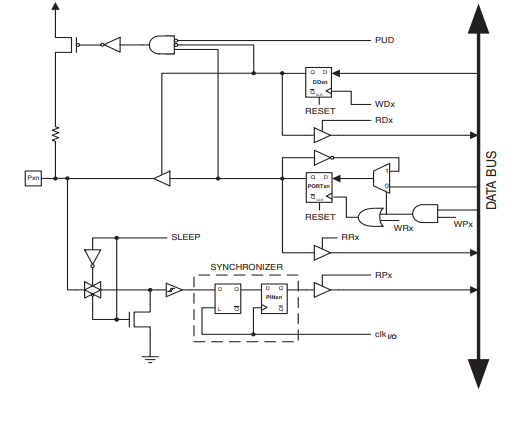
\includegraphics[width=.85\textwidth]{avr-pin-diag.png}
    \caption[Immagine ottenuta dal documento\cite{avr:m16u2}, fig. 12-2]{Diagramma funzionale dell'hardware relativo a un generico pin della famiglia AVR\cite[fig. 12-2]{avr:m16u2}}\label{fig:avr-pin}
\end{figure}

Alla scrittura del registro DDRx viene asserita la linea WDx, la quale salva lo stato del bit associato al pin nel flipflop pilotato da essa. Questo stato pilota un buffer che stabilisce se il pin stesso debba essere un input o un output.

In particolare, se lo stato salvato nel primo flipflop è 1, il pin sarà pilotato con livello logico pari allo stato salvato nel secondo flipflop in modo ``forte''.

Se invece lo stato del pin viene posto come input, ossia lo stato del primo flipflop è 0, è possibile pilotare il FET che alimenta la linea di pullup del pin. Questo accade perchè il segnale che rappresenta la direzione del pin è input negato della porta AND che controlla lo stato del pullup; per questo motivo, lo stato 0 permette alla porta di avere risultato 1 se lo stato del secondo flipflop è pari a 1, in quanto tale segnale sarebbe ignorato perchè il buffer di controllo è disabilitato.

La lettura dello stato del pin può avvenire in qualunque momento tramite la lettura del registro PINx, il quale asserisce la linea RPx e riporta lo stato salvato nello stadio di sincronizzazione.

La scrittura di tale registro viene reindirizzata al controllo del multiplexer in modo da poter invertire lo stato del pin senza averlo precedentemente letto, dimezzando la quantità di operazioni necessarie all'inversione dello stato.

Risulta quindi necessario stabilire due sequenze di operazioni per portare il pin da livello logico basso ``forte'' a livello logico alto ``debole''. In particolare la transizione da livello logico alto a livello logico basso deve avvenire precedentemente alla configurazione della direzione del pin. Questo garantisce che non vi siano possibilità di conflitti potenzialmente catastrofici, considerando il fatto che il segnale che determina l'attivazione del pullup è anche responsabile dello stato del pin. Questo problema risulta evitabile utilizzando un pullup esterno.

Analogamente per la conversione da livello logico basso a livello logico alto il cambio di stato dovrà avvenire successivamente al cambio di direzione.

Così facendo si riducono le possibilità di guasto e si minimizzano i tempi di incertezza --- considerando l'assenza di un pullup esterno --- i quali si limitano al tempo intercorso tra i due cambi di configurazione: ci sarà sempre un intervallo di tempo dove lo stato del pin sarà posto a livello logico basso e il pin posto in configurazione di input, lasciando così la connessione flottante.

In questi casi, data la durata di natura molto breve della commutazione e del periodo di incertezza, la capacitanza parassita della connessione permetterà di mantenere un livello logico costante.

\subsubsection{Implementazione del protocollo di comunicazione}

L'implementazione della comunicazione seriale emulata a livello software è soggetta a vincoli relativi al tempo di esecuzione.

L'implementazione si basa sull'utilizzo del timer TIMER1, un timer a 16 bit in grado di generare interrupt di comparazione e sul rilevamento della caduta da livello logico alto a basso per identificare un bit di inizio trasmissione.

Il concetto sul quale si basa il funzionamento consiste nel mantenere il timer in esecuzione ed eventualmente resettarne il conteggio nel caso si renda necessario una re-sincronizzazione in ricezione.

Entrambe le azioni di trasmissione e ricezione vengono implementate come una macchina a stati la quale iterazione è controllata dall'interrupt di comparazione di TIMER1.

Entrambe le funzionalità sono divide in due domini di esecuzione: l'esecuzione invocata dall'utente e la macchina a stati relativa eseguita con l'interrupt. 

La funzionalità di invio è implementata tramite un meccanismo di accodamento per due processi producer/consumer: alla prima invocazione della funzione di invio il byte viene salvato nella coda e viene abilitata la macchina a stati mostrata in figura~\ref{fig:phy-state-tx} tramite il flag \texttt{\_OD\_UART\_BUSY} la quale consumerà il dato al primo interrupt di comparazione, mentre nella seconda invocazione un secondo byte verrà inserito nella coda e la funzione potrà ritornare liberamente. 

È compito della macchina a stati riconoscere che un secondo byte è stato aggiunto alla coda \texttt{OD\_UART\_TX\_FULL} e di conseguenza essa inizierà una nuova trasmissione invece che andare allo stato \texttt{IDLE}.

\begin{figure}[t]
    \centering
    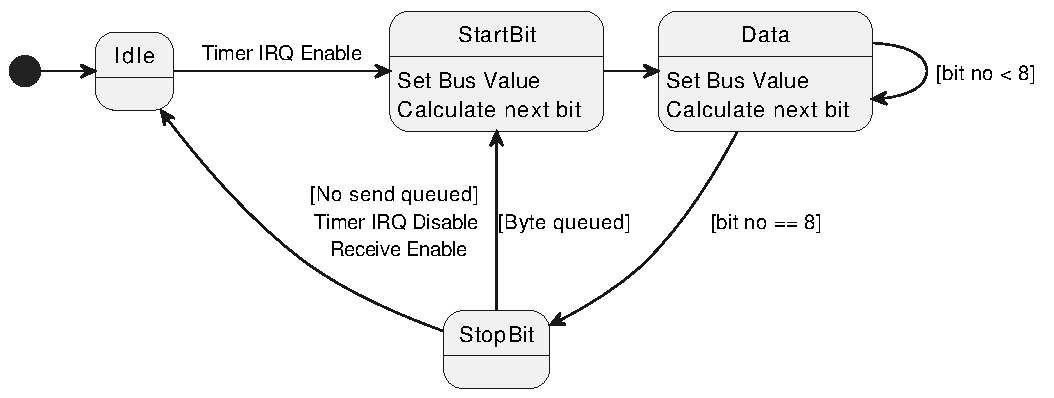
\includegraphics[width=.95\textwidth]{phy-tx-state.pdf}
    \caption[]{Macchina a stati per l'implementazione della trasmissione seriale}\label{fig:phy-state-tx}
\end{figure}

Il comportamento sopra descritto viene riassunto dalla figura~\ref{fig:phy-tx-timing}. Si noti come i cambiamenti di stato e il calcolo dei valori avvenga nell'iterazione precedente all'attuazione.
Inoltre l'immagine mostra come un eventuale aggiunta di un dato alla coda persista e venga indicata dal flag \texttt{OD\_UART\_TX\_FULL}.

Una volta terminata l'esecuzione dell'invio del dato, essendoci un ulteriore byte in coda, viene ripresa l'esecuzione immediatamente.

\begin{figure}[p]
    \checkoddpage%
    \ifoddpage%
        \begin{adjustbox}{addcode={\begin{minipage}{\width}}{\caption[]{%
            Diagramma delle tempistiche di esecuzione dell'invio di dati sulla linea seriale implementata via software.}\label{fig:phy-tx-timing}\end{minipage}},rotate=90,center}
            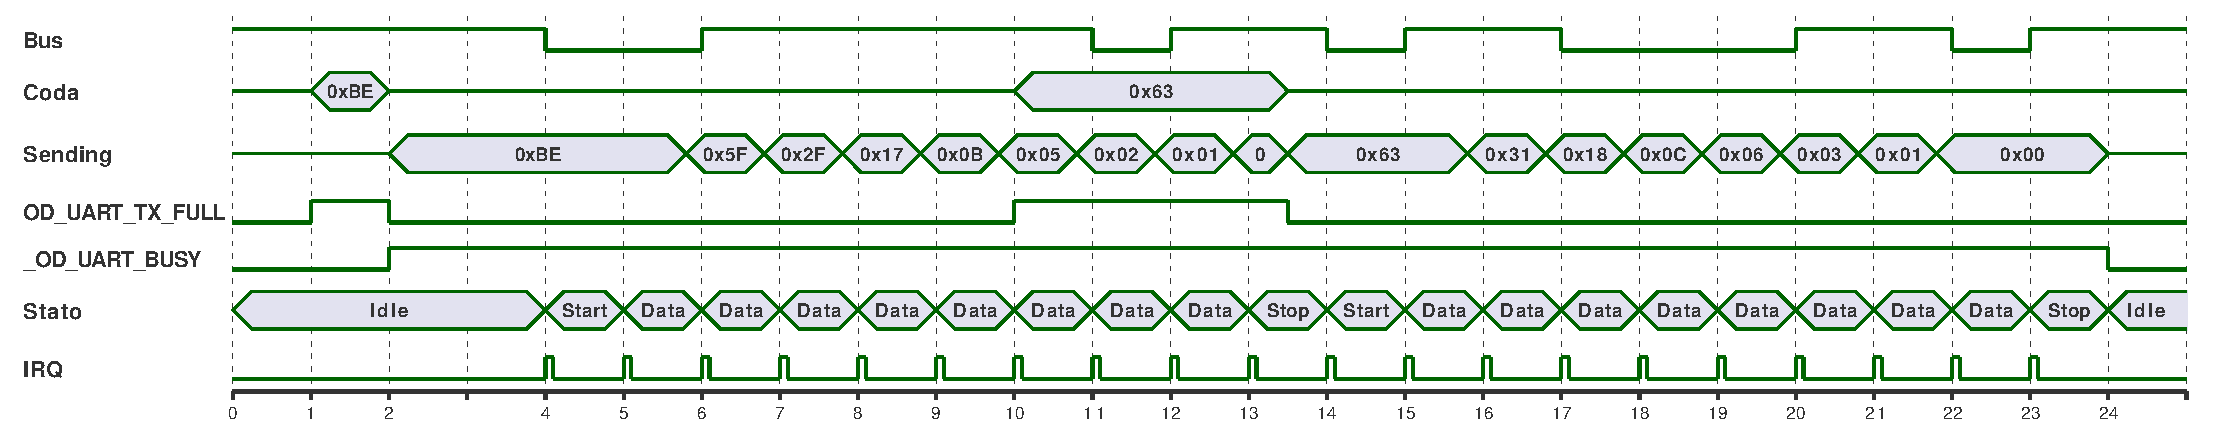
\includegraphics[width=\textheight]{phy-tx-timing.pdf}%
        \end{adjustbox}
    \else
        \begin{adjustbox}{addcode={\begin{minipage}{\width}}{\caption[]{%
            Diagramma delle tempistiche di esecuzione dell'invio di dati sulla linea seriale implementata via software.}\label{fig:phy-tx-timing}\end{minipage}},rotate=-90,center}
            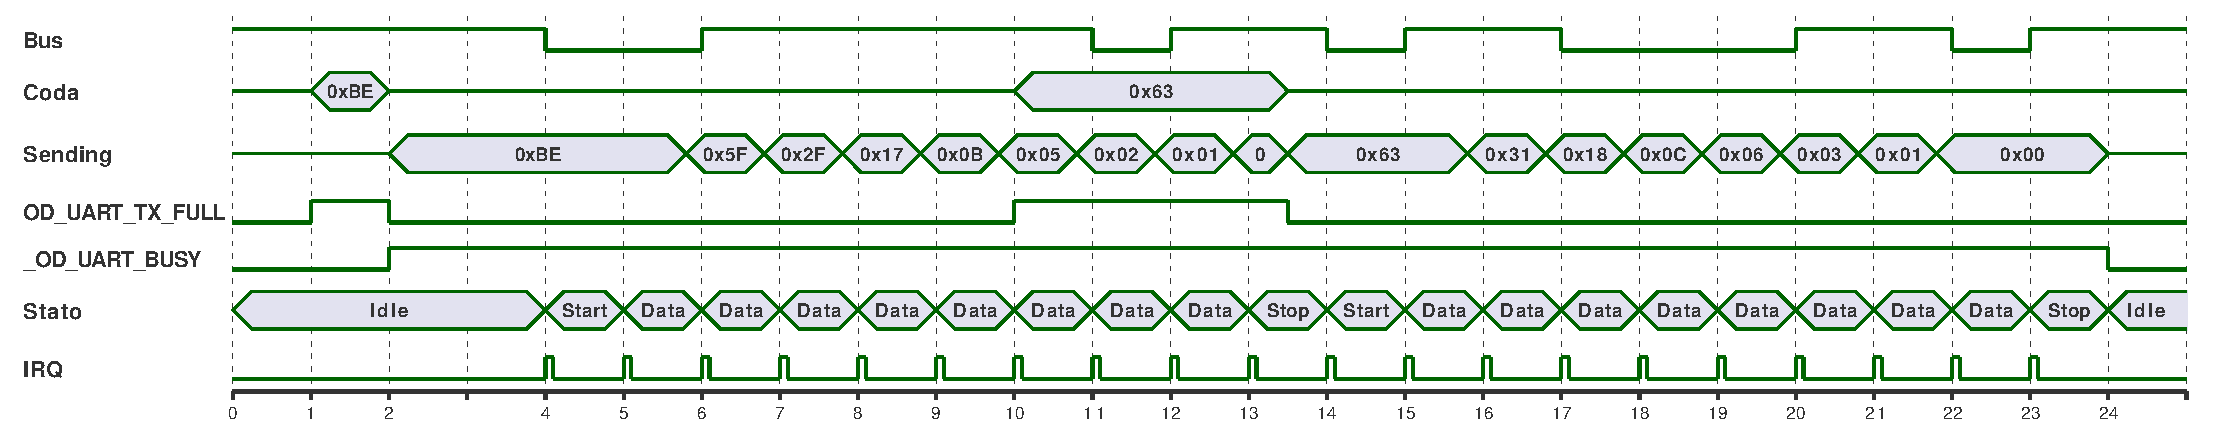
\includegraphics[width=\textheight]{phy-tx-timing.pdf}%
        \end{adjustbox}
    \fi
\end{figure}



La parte di ricezione viene implementata con una seconda macchina a stati mostrata in figura~\ref{fig:phy-rx-state} ma il primo passaggio di stato, da Idle a StartBit avviene alla ricezione di un interrupt relativo al cambiamento di stato del bus.

La ragione per cui questo passaggio debba avvenire all'avvenimento di un interrupt consiste nel fatto che il \textit{target} può inviare una risposta in qualsiasi istante temporale.

Risulta quindi necessario l'utilizzo di una struttura FIFO per il salvataggio dei dati ricevuti dalla quale poi l'utente potrà attingere durante l'esecuzione del software. In particolare il flag \texttt{\_OD\_UART\_AVAIL} indicherà la presenza di dati non ancora letti nel buffer.

Si rende quindi necessario poter ripristinare il conteggio del TIMER1 al fine di re-sincronizzare il clock di campionamento del bus al centro del bit per i motivi descritti nella sezione~\ref{ss:uart}, in particolare facendo riferimento all'equazione~\ref{eq:uart-period-receive-delay}. Questo comportamento è riassunto dalla figura~\ref{fig:phy-rx-timing}.

Alla ricezione dell'interrupt di cambio di stato la macchina a stati viene inizializzata e il timer resettato in modo che il successivo interrupt di comparazione avvenga a metà del bit successivo. Ad ogni interrupt il valore del bus viene aggiunto secondo l'equazione~\ref{eq:rx-push} al valore temporaneo fino al raggiungimento delle otto iterazioni. A questo punto lo stato passa a \texttt{StopBit}, dove il valore temporaneo viene inserito nella coda e viene asserito il flag \texttt{\_OD\_UART\_AVAIL}.

\begin{equation}\label{eq:rx-push}
    tmp_{i+1} = (bus << 7) | (tmp_i >> 1)
\end{equation}

\begin{figure}[p]
    \centering
    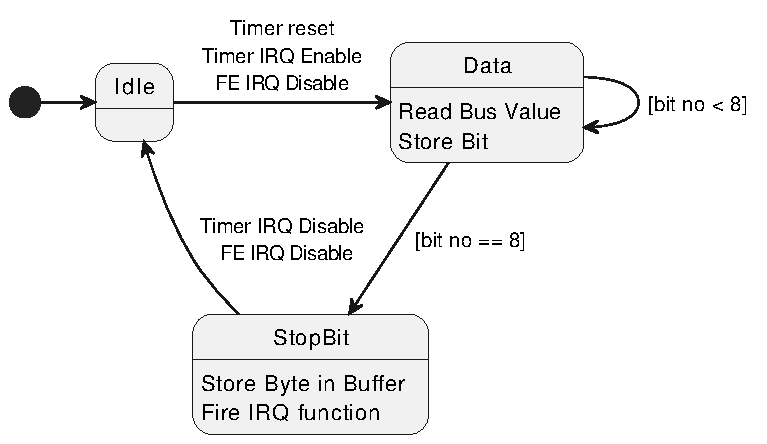
\includegraphics[width=.75\textwidth]{phy-rx-state.pdf}
    \caption[]{Macchina a stati relativa alla ricezione della seriale implementata in software.}\label{fig:phy-rx-state}
\end{figure}

\begin{figure}[p]
    \centering
    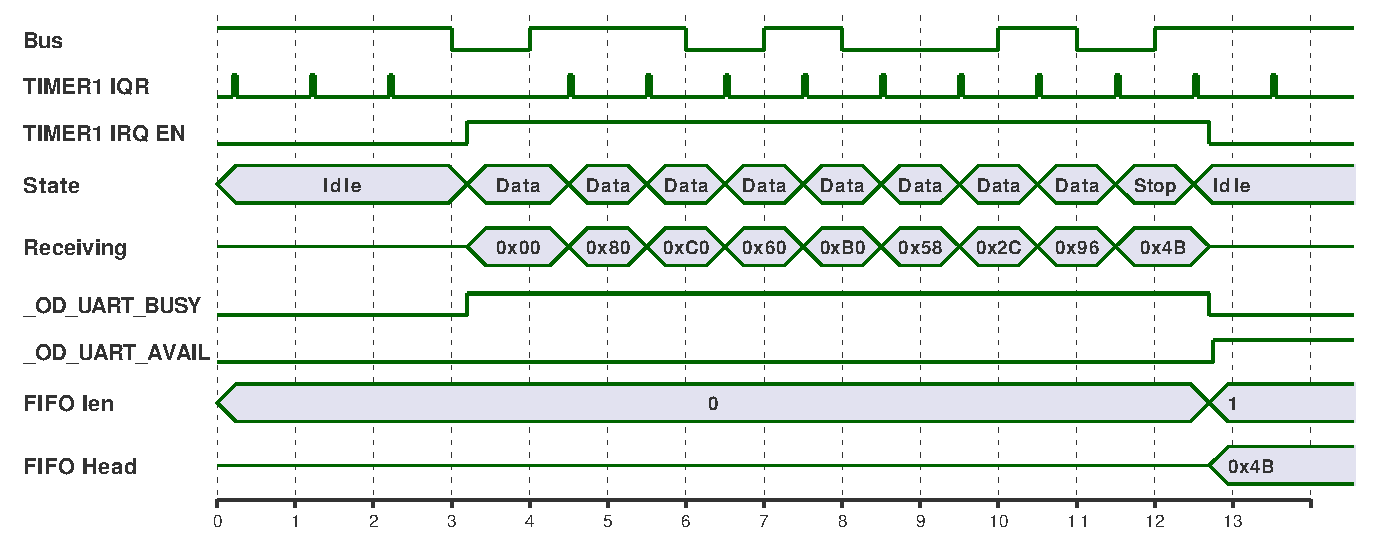
\includegraphics[width=.99\textwidth]{phy-rx-timing.pdf}
    \caption[]{Macchina a stati relativa alla ricezione della seriale implementata in software.}\label{fig:phy-rx-timing}
\end{figure}

Il listato~\ref{lst:fe-irq-management} mostra il frammento di codice per la gestione dell'inizio ricezione. 

\noindent\begin{minipage}{\textwidth}
    \begin{lstlisting}[style=C, caption={IRQ di gestione inizio trasmissione}, label=lst:fe-irq-management]
__attribute__((optimize("-Ofast"))) ISR(INT7_vect){
    cli();
    FE_IRQ_DISABLE(); //start a new rx. clear irq
    fast_flags = 0;
    uart_flags |= OD_UART_FLAG_BUSY_MASK; //set busy flag, reset flags
    TCNT1 = 0; //set counter to start at next bit. make correction for timer startup and bad things.
    TIMER_IRQ_ENABLE(); //enable timer and clear irq
    TIMER_IRQ_CLEAR();
    sei();
}
    \end{lstlisting}
\end{minipage}

È possibile osservare come nella compilazione dell'handler dell'interrupt venga privilegiata la velocità di esecuzione anziché lo spazio occupato dal compilato, e come il TIMER1 venga impostato a 0. Così facendo il campionamento avverrà verso l'inizio del bit inviato anziché alla metà del tempo di bit. 

Questo non è da considerarsi un problema data la bassa frequenza dell'insieme.

È inoltre necessario impostare \texttt{TCNT1 = OCR1A >\textcompwordmark> 2} nel caso si voglia utilizzare frequenze vicine a 125000 bit per secondo in quanto vanno considerati i tempi di esecuzione del codice e di reazione del timer. Questo valore è stato trovato sperimentalmente mediante l'uso di un analizzatore logico.